\section{The Proposed Algorithm}

The motivation behind the new algorithm is that EDA produces useful new genetic material when sampling it's probability model $M$, but fails to create anything new from the selected population, which is permitted to proceed into the next generation unaltered. By applying the principles of differential evolution, which only alter a chromosome if the alteration improves the individual, the selected population can be further improved before entering the next generation without risking any detrimental effects. Furthermore, the new algorithm will be able to approach problems from two perspectives at once, possibly enlarging it's area of applicability.

\begin{figure}[H]
  \centering
  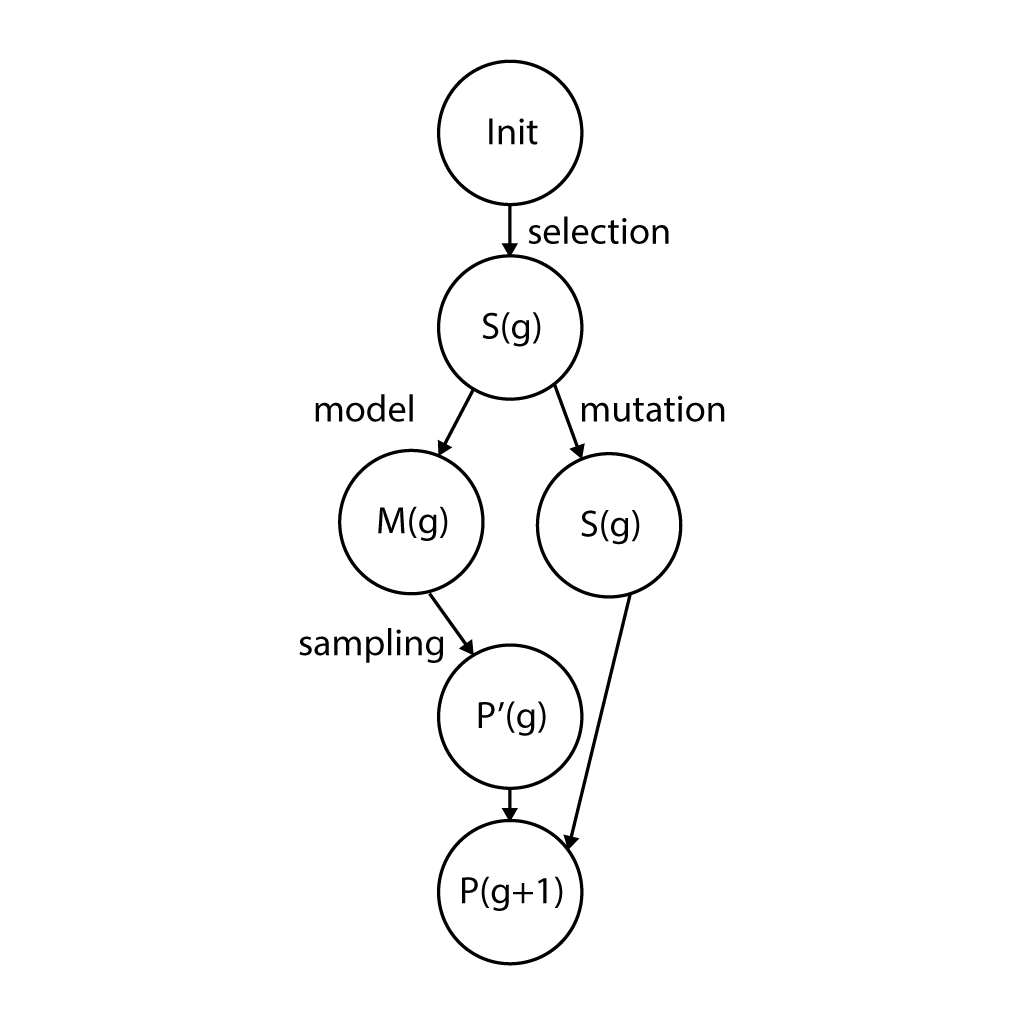
\includegraphics[width=.5\linewidth]{DEDA}
  \caption{Flow-diagram for algorithm}
  \label{fig:flowalg}
\end{figure}

The proposed improved algorithm, Differential Estimation of Distribution (DEDA), draws upon DE and EDA, applying differential mutation to the selected population of the EDA algorithm. The algorithm is described in algorithm~\ref{algo:my} and illustrated in figure~\ref{fig:flowalg}. The Matlab code can be viewed in appendix~\ref{appendix:algorithms}.


\begin{algorithm}[h]
  \caption{Proposed algorithm}
  \label{algo:my}
    \begin{algorithmic}
      \State $g\gets 0$
      \State $P(g)\gets \text{initialize population with size N}$
      \Repeat
        \State sort $P(g)$ by fitness
        \State $S(g)\gets \text{top t\% of P(g)}$
        \State $mn\gets \text{calculate mean vector by dimension from } S(g)$
        \State $std\gets \text{calculate standard deviation vector by dimension from } S(g)$
        \State $M(g)\gets \text{normal distribution created from } mn \text{ and } std$
        \State $P'(g)\gets \text{sample (100\%-t\%)*N individuals from M(g)}$

        \ForAll{Individuals $x$ in $S(g)$}
          \State Let $a$, $b$ and $c$ be three unique random individuals from $S(g)$ differing from $x$
          \State $v\gets a+(b-c)$
          \State $u\gets$ random blend of $x$ with $v$ (take at least 1 element from $v$)
          \If{$fitness(u) > fitness(x)$}
            \State $x\gets u$
          \EndIf
        \EndFor

        \State $P(g+1)\gets \text{merge } P'(g) \text{with } S(g)$
      \Until{Termination condition}
    \end{algorithmic}
\end{algorithm}

The algorithm belongs to the class of estimation of distribution algorithms, which use probability distributions to sample populations. Initially a population $P(0)$ is created by uniformly sampling values from a problem-specific parameter interval. Then the individuals in $P(g)$ (g stands for generation) are evaluated and the best solutions are selected into $S(g)$ (a threshold variable $t$ is used to determine how many solutions are selected, setting $t=50\%$ means that the best 50\% of the solutions are selected). A probabilistic model $M(g)$ is then constructed from the selected population $S(g)$. New individuals $P'(g)$ are sampled from $M(g)$. After the model $M(g)$ is constructed the individuals in $S(g)$ undergo differential mutation, cross-over and selection. Finally $P(g+1)$ is created by combining $S(g)$ with $P'(g)$. This procedure is repeated until the best solution in $P(g)$ is good enough or until a pre-determined number of evaluations/iterations is reached.
